\documentclass{article}

\usepackage{float}
\usepackage{hyperref}
\usepackage{graphicx}
\usepackage[notes,backend=biber]{biblatex-chicago}

\bibliography{main}
\begin{document}

\section{Alkoholkonsum in Baden Württemberg}


\subsection{Im vergleich zu anderen Bundesländern}
...

Wenn man allerdings die einzelnen Bundesländer genauer betrachtet fällt auf, dass in Bayern tatsächlich überdurchschnittlich viel Alkohol konsumiert wird \autocite{kraus_einfluss_2001}. In Baden Württemberg wird allerdings durchschnittlich relativ wenig Alkohol pro Tag getrunken. Auch der riskante Alkoholkonsum ist relativ gering. Da wir uns in unserer Seminararbeit hautpsächlich auf den Alkoholkonsum von Jugendlichen fokussieren wollen wäre eine Statistik zum durchschnittlichen Alkoholkonsum von Jugendlichen in den verschiedenen Bundesländern natürlich interessant. Bei unserer Rechere haben wir eine solche spezifische Statistik allerdings nicht gefunden. 

Um aber trotzdem eine Aussage über den Alkoholkonsum von Jugendlichen in Deutschland zu treffen, haben wir die Daten auf der Plattform GENESIS (Gemeinsames Neues Statistisches Informations-System) \autocite{noauthor_statistisches_nodate} verwendet. Auf GENESIS findet sich ein breit gefächertes Datenangebot von den statistischen Landesämtern und dem Statistischen Bundesamt. Dieses enthält u.a. einen Datensatz mit dem Bundesland, Alter, Geschlecht und der Hauptdiagnose aller Krankenhauspatienten in Deutschland \autocite{noauthor_genesis_nodate}. Aus dieser Statistik haben wir alle Krankenhausaufenthalte von Jugendlichen bis 19 Jahren, die aufgrund von einer Alkoholintoxikation (Diagnose ICD-10 F10.0 \autocite{noauthor_icd-10-code_nodate}) im Krankenhaus waren extrahiert. In der folgenden Grafik sieht man diese im Durchschnitt pro 100.000 Einwohner des jeweiligen Bundeslandes über die letzten 15 Jahre aufgelistet.

\begin{figure}[H]
    \centering
    \includegraphics[scale=.7]{"assets/Alkohol_Bundesländer_avg_15_Jahre.png"}
    \caption{Alkoholbedingte Krankenhausaufenthalte von Jugendlichen in Abhängigkeit des Bundeslandes}
    \label{fig:Krankenhausaufenthalte_1}
\end{figure}

Für die Bevölkerungsanzahlen zur normalisierung der Statistik wurde die Bevölkerung des jeweiligen Bundeslandes zum jeweiligen Zeitpunkt verwendet \autocite{noauthor_statistisches_2024}. Die Werte wurden mit Python berechnet und die Grafik wurde mit der Python Bibliothek Matplotlib \autocite{noauthor_matplotlib_nodate} erstellt. 

Es fällt auf, dass die Werte für kleine Bundesländer (Saarland, Hamburg und Berlin) stark abweichen. Das könnte an den geringen Fallzahlen liegen, die dann zu Extremwerten führen. Die absoluten Fallzahlen schwanken im zum Beispiel Saarland über die Jahre von 200 bis knapp 400. Ein weiterer wichtiger Aspekt, der bei der Analyse dieser Daten beachtet werden muss, ist der Länderaustausch von Patienten. Das Bundesland, in dem ein Patient behandelt werden muss, muss nicht mit dem Wohnort des Patienten übereinstimmen. Das kann aufgrund der normalisierung der Daten zu einer verfälschung der Ergebnisse führen. Auf GENESIS ist auch eine Statistik verfügbar, die statt dem Ort des Krankenhauses den Wohnort der Patienten angibt \autocite{noauthor_genesis_nodate-1}.

\begin{figure}[H]
    \centering
    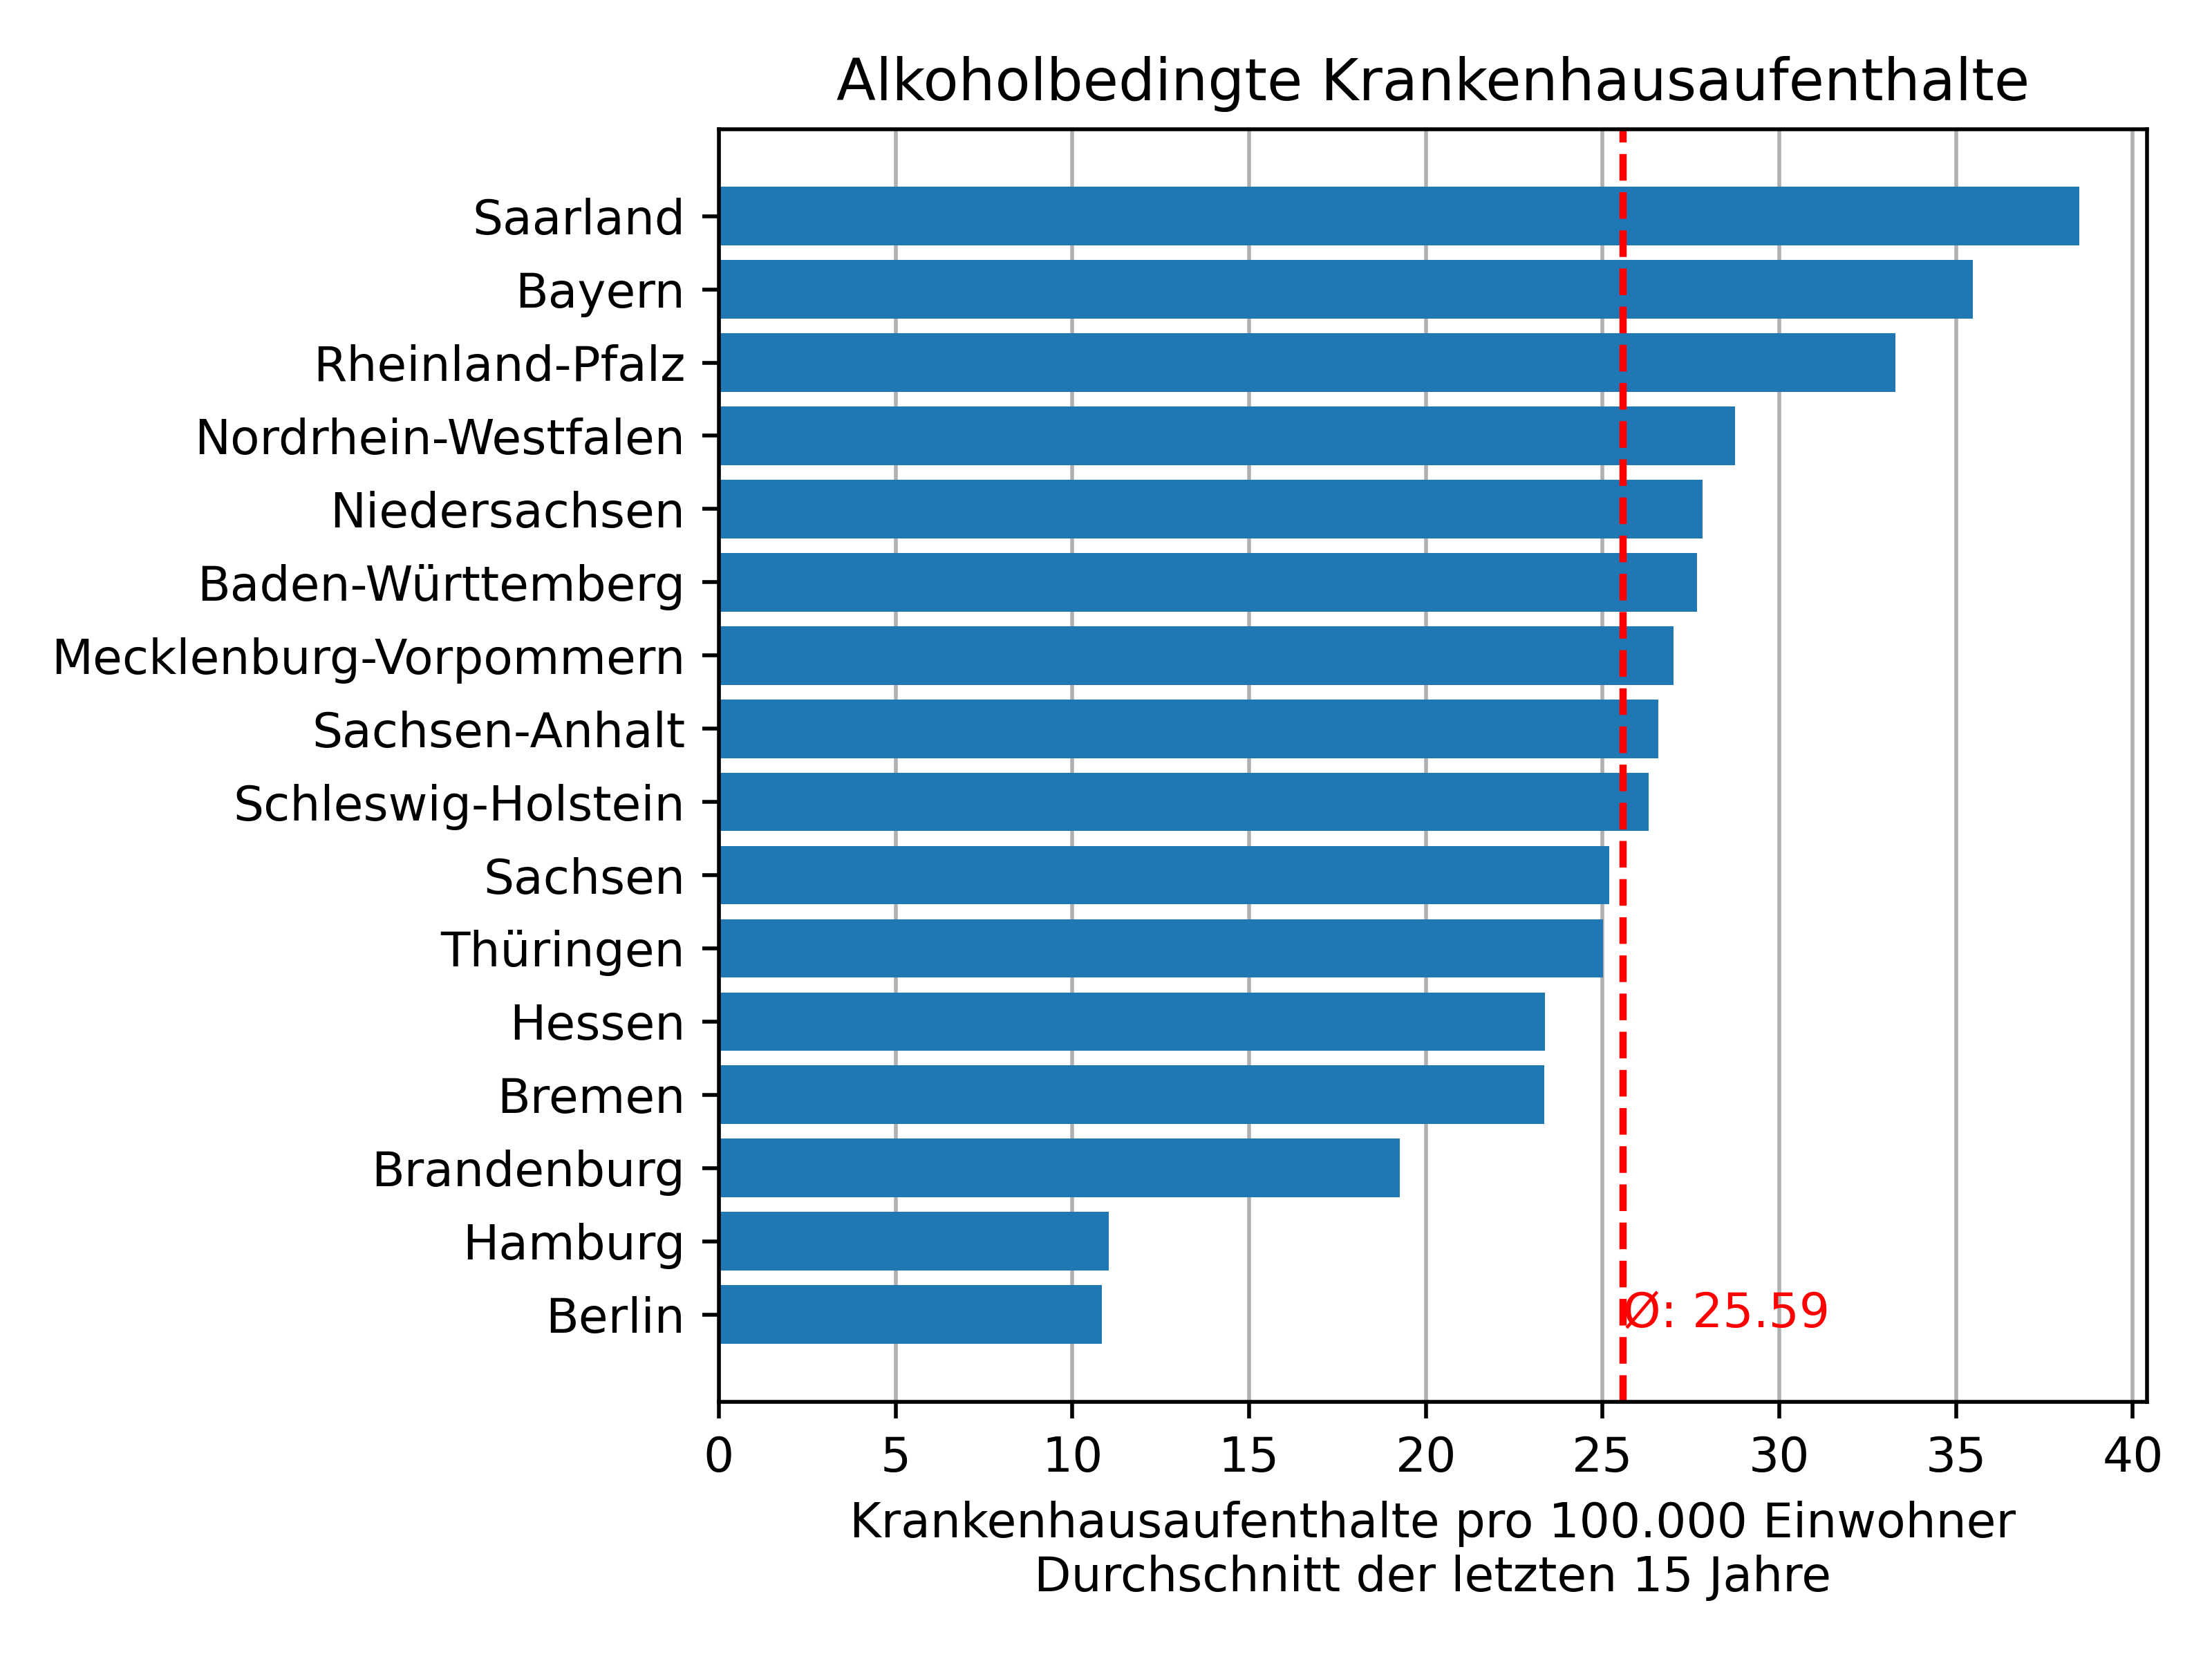
\includegraphics[scale=.7]{"assets/Alkohol_Wohnort_avg_15_Jahre.png"}
    \caption{Alkoholbedingte Krankenhausaufenthalte von Jugendlichen in Abhängigkeit des Wohnortes}
    \label{fig:Krankenhausaufenthalte_2}
\end{figure}

\ref{fig:Krankenhausaufenthalte_1} wurde mit den gleichen Methoden wie \ref{fig:Krankenhausaufenthalte_2} erstellt. Patienten deren Wohnort unbekannt ist und Patienten, die aus dem Ausland kommen wurden ignoriert. 
Die Werte für die meisten größeren Bundesländer sind nahezu gleich geblieben, da dort der Anteil der Patienten, die in einem anderen Bundesland behandelt wurden im vergleich zu den Patienten, die in ihrem Heimatbundesland behandelt wurden sehr klein ist. Die Werte der kleineren Bundesländer (Hamburg, Berlin, Bremen und Saarland) sind dagegen stärker gesunken, vor allem bei Bremen. Das könnte daran liegen, dass ein Teil der Patienten, die zum Beispiel in einem Krankenhaus in Bremen behandelt wurden aus dem umliegenden Niedersachsen kommen. Dass die hohen Werte im Saarland kein Fehler in der Statistik sind, sondern ein reales Problem darstellen zeigt sich auch in diesem Artikel \autocite{noauthor_saarland_nodate}, der das Problem des alkoholmissbrauchs von Jugendlichen im Saarland beschreibt. 
\\\\\\
\printbibliography
\end{document}
